\documentclass[11pt,a4paper]{report}
\usepackage[utf8]{inputenc}
\usepackage[french]{babel}
\usepackage[T1]{fontenc}
\usepackage{amsmath}
\usepackage{amsfonts}
\usepackage{amssymb}
\usepackage{graphicx}
\usepackage{lmodern}
\usepackage{xlop}
\usepackage{fullpage}
\usepackage{minted}

\author{Sylvain Julmy}
\title{Cryptographie : Résumé}

\setlength{\parindent}{0cm}

% Python
\newminted{python}{frame=single, framesep=6pt, breaklines=true, fontsize=\scriptsize}
\newmintedfile{python}{frame=single, framesep=6pt, breaklines=true, fontsize=\scriptsize}

\begin{document}

\maketitle

\section*{Corps $\mathbb{F}_{2^\nu}$}

$\nu = 4$,polynôme irréductible primitif

$m(x) = x^4+x+1 \in \mathbb{F}_2[x]$ de degré $\nu$

Si le produit scalaire du mot reçus $r$ est linéairement indépendant de chaque ligne de $H$, alors $r$ appartient au code.

\section*{Série 7}

\subsection*{(1)}

\subsection*{(2)}
$x^8+x^7+x^2+x+1$ est un polynôme irréductible de primitif de $\mathbb{F}_2[x]$.
\paragraph*{(a)} Vérifier que $\alpha^8$ et $\alpha^9$ sont correct :
\begin{itemize}
\item[$\bullet$] $\alpha^8 = \alpha^7+\alpha^2 + \alpha + 1 = 10000111_2 = 135_{10} \rightarrow\\ \alpha^7 = 128_{10} = 10000000_2, \alpha^2 = 4_{10} = 00000100_2\\
\alpha = 2_{10} 00000010_2, 1 = 1_{10} = 00000001_2 \rightarrow \\
\alpha^7\oplus\alpha^2 \oplus \alpha \oplus 1 =
100000111_2 = 128 + 4 + 2 + 1 = 135_{10} = \alpha^8$

\item[$\bullet$] $\alpha^9 = 137_{10} = 10001001_2 = 10000000_2 \oplus 00001000 \oplus 00000001 = 128_{10} + 8_{10} + 1_{10} = \alpha^7 + \alpha^3 + 1$

\item[$\bullet$] Exemple avec $\alpha^{20} = 236_{10} = 11101100_2 = \alpha^7+\alpha^6+\alpha^5+\alpha^3+\alpha^2$
\end{itemize}

Il suffit de combiner les éléments primitifs : ${1,\alpha,\alpha^2,\alpha^3,\alpha^4,\alpha^5,\alpha^6,\alpha^7}$ avec l'opérateur XOR $\oplus$.

\subsection*{(3)}

\subsection*{(4)}

\subsection*{(5)}

\subsection*{(6)}

\subsection*{(7)}

\chapter{Historiques}

\chapter{Chiffrement symétrique}

\section{Chiffrement par flot}

\subsection{One-time pad}

Soit un message $x$ de $l$ bits, on génère une clef de $l$ bits complètement aléatoire. On transmet la clef à Bob et on calcule le texte chiffré $y=x\oplus k$, où $\oplus$ est un XOR. Ce code est parfaitement sûr.

Un chiffrement est dit parfaitement sûr si le texte clair $x$ et le texte chiffré $y$ sont statistiquement indépendant:
$$ P[X|Y] = P[X] $$
Ce qui vaut
$$ P[X|Y] = \frac{P[X \wedge Y]}{P[Y]} $$

Démonstration :
\begin{align*}
P[X = x \wedge Y = y] &= P[X=x \wedge K = x \oplus y] \\
                      &= P[X=x] \cdot P[K=x \oplus y] \\
                      &= P[X=x] \cdot 2^{-l}
\end{align*}

\begin{align*}
P[Y = y] &= \sum_x P[X=x \wedge Y = y] \\
         &= \sum_x P[X=x] \cdot 2^{-l} \\
         &= 2^{-l} \sum_x P[X=x]\\
         &= 2^{-l}
\end{align*}

Finalement

\begin{align*}
P[X=x | Y=y] &= \frac{P[X=x \wedge Y=y]}{P[Y=y]} \\
             &= \frac{P[X=x] \cdot 2^{-l}}{2^{-l}} \\
             &= P[X=x]
\end{align*}

Inconvénient : clef unique, le texte chiffré peut être manipulé, la transmission des clefs posent problèmes et la génération d'une clef aléatoire est problématique.

\subsection{RC4}

RC4 n'est pas recommandé en pratique, on initialise une clé puis on utilise un générateur de flot pseudo-aléatoire en essayant de reproduire le "one-time pad".
\begin{listing}[H]
\caption{Initialisation de la clef}
\begin{pythoncode}
for i from 0 to 255 :
    S[i] = i

j = 0
for i from 0 to 255 :
    j = (j + S[i] + key[i mod key.length]) mod 256
    swap(S[i],S[j])
\end{pythoncode}
\end{listing}

\begin{listing}[H]
\caption{Génération du flux}
\begin{pythoncode}
i = 0
j = 0
while generatingOutput :
    i = (i + 1) mod 256
    j = (j + S[i]) mod 256
    swap(S[i],S[j])
    K = S[S[i] + S[j]) mod 256
    output K
\end{pythoncode}
\end{listing}

\subsection{Grain}

Algorithme qui prend une clef de 80 bits et un vecteur d'initialisation de 64 bits. Économe en ressource si implémenter sur FPGA et encore incassé à ce jour.

\begin{center}
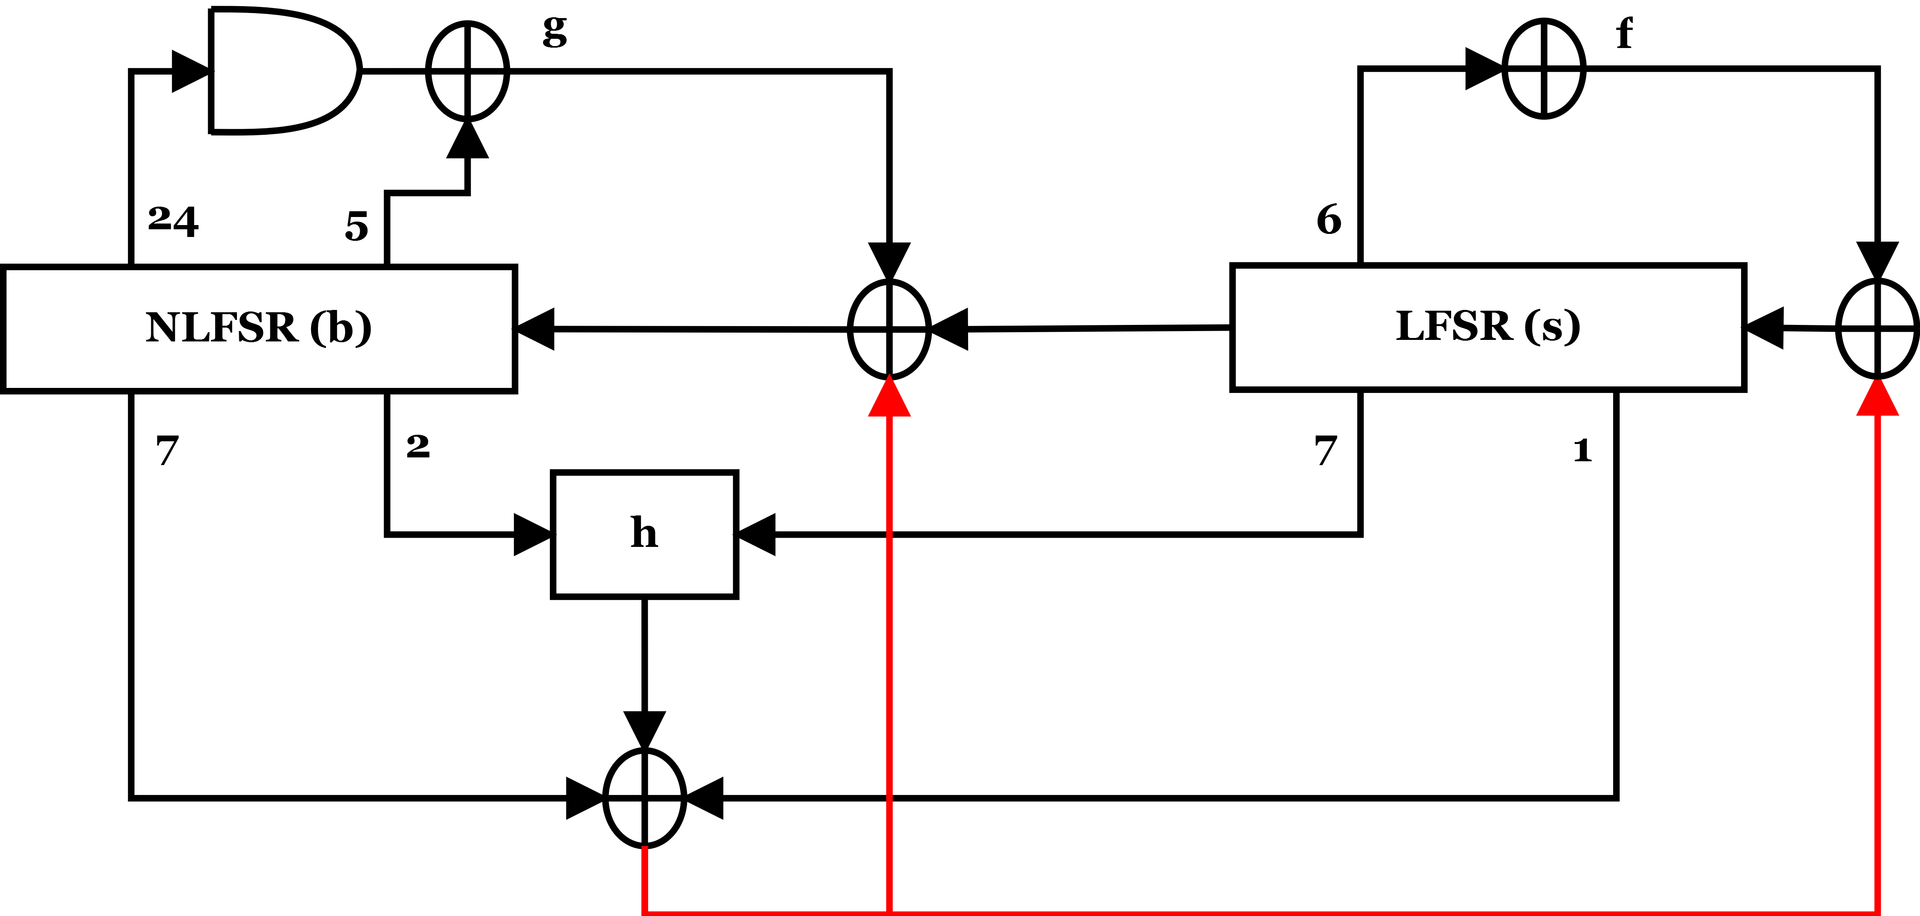
\includegraphics[width=0.98\textwidth]{img/Grain_init.png}
\end{center}

\section{Chiffrement par bloc}

Étant donné un chiffrement par bloc $F$ qui chiffre des textes clairs $X = \{x_1,...,x_l\}$ de $l$ bits au moyen d'une clef $K$, où $x_i \in \mathbb{Z}_2$, on peut écrire $F$ sous la forme d'un système d'équations booléennes :
\begin{align*}
&y_1 = F^1_K(x_1,...,x_l) \\
&... \\
&y_l = F^l_K(x_1,...,x_l)
\end{align*}

Confusion : les fonctions $F^1_K,...,F^l_K$ doivent être mathématiquement complexes car en pratique on peut trouver la clef $K$ au moyen du texte clair et du texte chiffré. Les fonctions ne doivent pas être linéaire.

Diffusion : Une modification d'un seul bit du texte clair devrait changer en moyenne la moitié des bits du texte chiffré.

\subsection{Recherche exhaustive de clef}

Le principe est d'essayer toutes les clefs possibles. La recherche exige un critère d'arrêt : comment savoir que la clef est bonne ? Pour une clef de $l$ bits, il faut au minimum $1$ essai, au pire des cas $2^l$ essais et en moyenne $2^{l-1}$ essais. En 2015, une taille de clef de $64$ bits est considéré comme insuffisante. $80$ bits en minimal. Moore : la puissance de calcule double environ tous les 18 mois.

\subsection{Chiffrement itéré}

Itérer une fonction de ronde un certain nombre de fois. Chaque fonction de ronde prend comme paramètre un sous-clef de la clef principale au moyen de cadencement de clef. Le but est de trouver un équilibre entre nombre d'itération et force du code.

\subsection{DES}

Prend une clef de $64$ bits dont $8$ bits ignorés (donc $56$ bits) et est bâti sur un schéma de Feistel à $16$ rondes.

$IP$ est une matrice de permutation sur $\mathbb{Z}_2$ de taille $64 \times 64$ et $FP$ est son inverse. $E$ est une fonction linéaire qui étend son entrée de $32$ bits en une sortie de $48$ bits en dupliquant certains bits. $P$ est une matrice de permutation de $32 \times 32$. $PC1$ est une fonction linéaire qui passe de $64$ bits à $56$ bits. $PC2$ est une fonction linéaire qui passe de $56$ bits à $48$ bits

\subsection{Triple DES}

Triple DES à deux clefs  : $Y = DES_{K1}(DES_{K2}^{-1}(DES_{K1}(X)))$ \\
Triple DES à trois clefs : $Y = DES_{K3}(DES_{K2}^{-1}(DES_{K1}(X)))$

\subsection{IDEA}

Possède une clef de $128$ bits, sa fonction de ronde est itérée $8.5$ fois et qui chiffre des blocs de données de $64$ bits. IDEA repose sur l'utilisation de 3 opérations incompatibles algébriquement :
\begin{itemize}
    \item l'addition sur $\mathbb{Z}^{16}_2$ notée $\oplus$
    \item l'addition sur $\mathbb{Z}_{2^{16}}$ notée $\boxtimes$
    \item la multiplication sur $\mathbb{Z}_{2^{16}+1}$, notée $\odot$ et où $0$ est identifié à la valeur $2^{16}$.
\end{itemize}

IDEA est basé sur un schéma de Lai-Nassem.

\subsection{AES}

Chiffre des données de $128$ bits qui supporte des clefs de $128$ bits (10 rondes), $192$ bits (12 rondes) et $256$ bits (14 rondes). Très efficace sur les plateformes embarquées, CPU et hardware.

\chapter{Modes Opératoires et Authentification on Symétrique}

\section{Mode opératoire}

Un algorithme de chiffrement par flot peut chiffrer des données de n'importe quelle longueur contrairement à un algorithme de chiffrement par bloc (64 ou 128 bit typiquement).

Un mode opératoire est une manière de chiffrer des données plus grandes que la taille d'un bloc. Modes classiques :
\begin{itemize}
    \item "Electronic Code Block" ECB
    \item "Cipher Block Chaining" CBC
    \item "Counter Mode" CTR
    \item CFB, OFB,...
\end{itemize}

\subsection{ECB}

Les données à chiffrer sont divisées en blocs de la taille du bloc de l'algorithme de chiffrement, chaque bloc est chiffré indépendamment des autres.

\paragraph*{Problème : } Deux blocs de textes clairs identiques seront chiffrés de manières identiques. On a donc une perte potentielle de confidentialité. Le mode ECB résiste donc très mal aux attaques visant à modifier l'intégrité du texte chiffré. C'est un algorithme déterministe.

\subsection{CBC}

\paragraph*{Principe : }
\begin{itemize}
    \item les données sont divisées en blocs de la taille du bloc de l'algorithme de chiffrement
    \item avant le chiffrement, un bloc est combiné avec un XOR avec le texte chiffré précédent
    \item Le premier bloc est combiné avec un bloc de chiffrement aléatoire appelé \textbf{vecteur d'initialisation} (IV)
\end{itemize}

Chaque bloc de texte chiffré est dépendant de tous les blocs précédents. Le chiffrement est séquentiel mais le déchiffrement peut être parallèle.

\subsection{CTR}

\begin{itemize}
    \item Un compteur est chiffré par l'algorithme de chiffrement par bloc
    \item Le flux est combiné au moyen d'un XOR avec le texte clair
\end{itemize}

Algorithme parallèle, pas besoin de couper des données si pas de la bonne taille, la sécurité repose sur la qualité de l'IV, mauvaise résistance aux adversaires attaquant l'intégrité du texte chiffré.

\section{Fonction de hachage}

Fonction définis comme $H:\{0,1\}* \rightarrow \{0,1\}^l$ qui possède les propriétés suivantes :
\begin{itemize}
    \item le calcul de l'empreinte (digest) $h = H(m)$ d'une message $m$ est une opération rapide
    \item étant donnée une image $h$, il est impossible en pratique de trouver un message $m$ tel que $h=H(m)$ (\textbf{résistance à la première préimage})
    \item étant donnée un message $m$ et son empreinte $h=H(m)$, il est impossible en pratique de trouver un message $m'\neq m$ tel que $h=H(m')$ (\textbf{Résistance à la seconde préimage})
    \item Il est impossible en pratique de trouver deux messages $m \neq m'$ tels que $H(m) = H(m')$
\end{itemize}

\subsection{Construction de Merkle-Damg$\dot{\text{a}}$rd}

Cette construction permet de transformer une fonction de compression en une fonction de hachage.

\begin{center}
    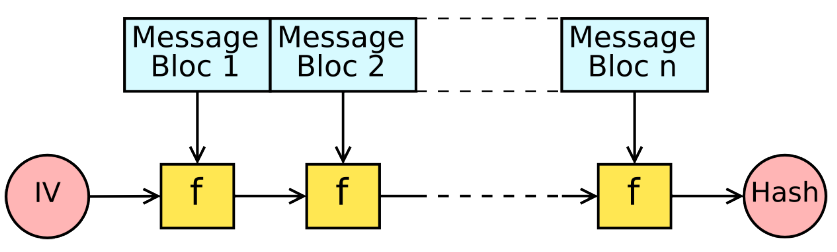
\includegraphics[width=0.5\textwidth]{img/merkle_damgard.png}
\end{center}

\subsection{Construction de Davies-Meyer}

La construction de Davies-Meyer permet de transformer un algorithme de chiffrement par bloc en une fonction de compression.

\begin{center}
    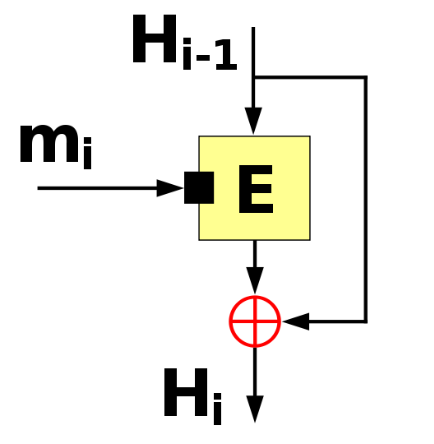
\includegraphics[width=0.3\textwidth]{img/davies_meyer.png}
\end{center}

\subsection{Quelques fonctions de hachage}

\begin{description}
    \item[MD5] : Empreintes de 128 bits, \textbf{cassée ! } Il est théoriquement possible de trouver des collisions en quelques secondes
    \item[SHA-1] : Empreintes de 160 bits, \textbf{cassée ! } Il théoriquement possible de trouver des collisions en environ $2^64$ opérations
    \item[SHA-256, SHA-512] : Empreintes de 256 et 512 bits et "sûre"
    \item[SHA-3] : Empreintes de 256 et 512 bits, similaire à AES
\end{description}

\section{Authentification symétrique}

La cryptographie symétrique peut garantir l’authenticité d’un canal de communication

une famille de fonction est définis comme $h_k:\{0,1\}* \times \kappa \longrightarrow \{0,1\}^l$. A éviter : $SHA256(X) \oplus K$. Exemple de familles sûre : HMAC, CBC-MAC,...

\paragraph*{Protocole : }
\begin{enumerate}
    \item Alice et Bob partage un secret $K$
    \item Alice envoie la liste $X$ ainsi que la valeur de MAC $\tau = h_k(X)$ à Bob
    \item Bob calcule $\tau = h_k(X')$ avec le message $X'$ reçu, et l'accepte comme étant authentique $\Longleftrightarrow \tau = \tau'$ où $\tau'$ est la valeur du MAC attaché au message.
\end{enumerate}

\subsection{HMAC}

Construit un MAC à partir de n’importe quelle fonction de hachage cryptographiquement sûre, HMAC-MD5 et HMAC-SHA1 sont très largement utilisées en pratique (TLS, IPSec, ...).

\begin{align*}
& \text{Fonction de hachage } H \\
& \text{Clef secrète } K \\
& \text{Message à authentifier } X \\
& \text{Constantes } opad = 0x5c5c5c...5c \ ipad = 0x363636363...36 \\
& \\
& HMAC_k(X) = H((K\oplus opad)||H((K\oplus ipad)||X))
\end{align*}

\subsection{CBC-MAC}

Seulement sûr pour des messages de taille fixe !

\begin{center}
    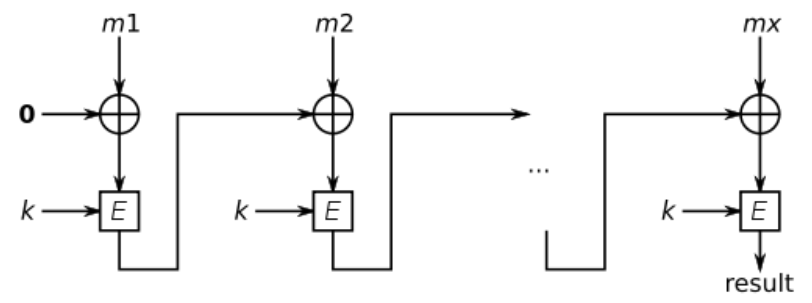
\includegraphics[width=0.6\textwidth]{img/cbc_mac.png}
\end{center}

\section{Exercices}

\paragraph*{1.1 : } Sur un réseau à $l$ nœuds, il faut $\frac{n(n-1)}{2}$.
\begin{itemize}
    \item[$l=10$      :] $0.5\cdot10\cdot9=45$  
    \item[$l=1000$    :] $0.5\cdot1000\cdot999=49500$
    \item[$l=7500000$ :] $0.5\cdot7500000\cdot7499999\approx2.8\cdot10^{13}$
\end{itemize}

\paragraph*{1.2 : } Dans le cas du chiffrement asymétrique, on ne peut pas déchiffrer le message avec la clé utiliser pour le chiffrer. Il s'agit d'une fonction à sens unique. Cela veut dire que n'importe quelle personne qui possède la clef publique peut chiffré un message mais seulement celui qui à la clef privée peut le déchiffrer. Donc pas besoin de partager de clefs.

\paragraph*{1.3 : } La clef publique ne doit pas être trivial. Par exemple, dans le cas de RSA, le clef publique est composé, en partie, d'un nombre $n$ qui est le produit de deux nombres premiers très grand $n = pq$. Si $n$ est petit, on est capable de trouver relativement rapidement sa décomposition en facteur premier et donc de déchiffrer le message.  Plus généralement, la clef publique contient l'information nécessaire à déchiffrer le message mais le temps nécessaire pour le faire est trop grand. Dans le cas de RSA, par ailleurs, ne pas choisir le carré d'un nombre premier.

\paragraph*{1.4 : } Prenons par exemple la clef publique suivante : $(n=86701,e=919)$. On sait que un des nombres de la décomposition en facteur premier est inférieur à $\sqrt{n} = 294$. On doit donc juste tester si un nombre entre $2$ et $294$ divise $n$. Ce qui nous donne $293$ opérations modulo à faire jusqu'à trouver $n \equiv 0 \mod n$. On à donc la complexité de la décomposition en facteur premier : $O(\sqrt{n})$ pour $n$ facteur de deux nombres premiers. Si $n$ est assez grand, le nombre d'opération également.

\paragraph*{1.5 : } Alice va utiliser la clef publique de Bob pour chiffrer le message et Bob va utiliser sa clef privé pour le déchiffrer.

\paragraph*{2.1 : } Le groupe $\mathbb{Z}^*_{17}$ possède $16$ éléments : $Z^*_{17} = \{1,2,3,4,5,6,7,8,9,10,11,12,13,14,15,16\}$
 
\paragraph*{2.2 : }
\begin{pythoncode}
for i in range(1, 25):
    print str(i) + "^3 mod 17 = " + str(3**i % 17)
\end{pythoncode}

Output :

\begin{verbatim}
1^3 mod 17 = 3   2^3 mod 17 = 9   3^3 mod 17 = 10  4^3 mod 17 = 13
5^3 mod 17 = 5   6^3 mod 17 = 15  7^3 mod 17 = 11  8^3 mod 17 = 16
9^3 mod 17 = 14  10^3 mod 17 = 8  11^3 mod 17 = 7  12^3 mod 17 = 4
13^3 mod 17 = 12 14^3 mod 17 = 2  15^3 mod 17 = 6  16^3 mod 17 = 1
17^3 mod 17 = 3  18^3 mod 17 = 9  19^3 mod 17 = 10 20^3 mod 17 = 13
21^3 mod 17 = 5  22^3 mod 17 = 15 23^3 mod 17 = 11 24^3 mod 17 = 16
\end{verbatim}

On remarque que tous les nombres éléments de $\mathbb{Z}^*_{17}$ sont présent.

\paragraph*{2.3 : } L'ordre de $\mathbb{Z}^*_{17}$ pour $x=3$ est $16$ : $3^16 \equiv 1 \mod 17$. L'ordre de $\mathbb{Z}^*_{17}$ pour $x=2$ est $8$ : $2^8 \equiv 1 \mod 17$.

\begin{pythoncode}
for j in range(1,17):
    for i in range(1, 26):
        order = j**i % 17
        if order == 1:
            print "order for x = " + str(j) + " : " + str(i)
            break
\end{pythoncode}

\begin{verbatim}
order for x = 1 : 1   order for x = 2 : 8   order for x = 3 : 16
order for x = 4 : 4   order for x = 5 : 16  order for x = 6 : 16 
order for x = 7 : 16  order for x = 8 : 8   order for x = 9 : 8 
order for x = 10 : 16 order for x = 11 : 16 order for x = 12 : 16
order for x = 13 : 4  order for x = 14 : 16 order for x = 15 : 8
order for x = 16 : 2
\end{verbatim}

Les éléments dont l'ordre est maximal sont des générateurs car $\forall g_i \in \mathbb{Z}^*_m$, les éléments élevé à chaque puissance $g_i$ donne chaque élément de $\mathbb{Z}^*_m$.

\paragraph*{2.4 : }
\begin{pythoncode}
# compute generator for field Z*_p
def compute_generator(p, max_i):
    res = []
    for i in range(1, p):
        for j in range(1, max_i + 1):
            order = (i ** j) % p
            if order == 1:
                if j == p - 1:
                    res.append(i)
                break
    return res

def discret_logarithm(x, p):
    generators = compute_generator(p, p + 1)
    for g in generators:
        for y in range(1,1000):
            if x == ((g**y) % p):
                return (g,y)


# Compute discret logarithm for all element in Z*_17
for element in range(1,17):
    print "discret logarithm of " + str(element) + " : " + str(discret_logarithm(element,17))
\end{pythoncode}
\begin{verbatim}
discret logarithm of 1 : (3, 16) discret logarithm of 2 : (3, 14)
discret logarithm of 3 : (3, 1)  discret logarithm of 4 : (3, 12)
discret logarithm of 5 : (3, 5)  discret logarithm of 6 : (3, 15)
discret logarithm of 7 : (3, 11) discret logarithm of 8 : (3, 10)
discret logarithm of 9 : (3, 2)  discret logarithm of 10 : (3, 3)
discret logarithm of 11 : (3, 7) discret logarithm of 12 : (3, 13)
discret logarithm of 13 : (3, 4) discret logarithm of 14 : (3, 9)
discret logarithm of 15 : (3, 6) discret logarithm of 16 : (3, 8)
\end{verbatim}

\paragraph*{3.1 : } Le groupe multiplicatif $\mathbb{Z}^*_{77}$ contient $76$ éléments : $\{1,2,...,76\}$. Le groupe multiplicatif $\mathbb{Z}^*_{pq}$ contient $pq-1$ éléments en général.

\paragraph*{3.2 : }
\begin{pythoncode}
res = []
for x in range(1,21):
    res.append(x**7 % 77)
\end{pythoncode}
\begin{verbatim}
[1, 51, 31, 60, 47, 41, 28, 57, 37, 10, 11, 12, 62, 42, 71, 58, 52, 39, 68, 48]
\end{verbatim}

\paragraph*{3.3 : }
\begin{pythoncode}
res2 = []
for element in res:
    res2.append(element**43 % 77)
\end{pythoncode}
\begin{verbatim}
[1, 2L, 3L, 4L, 5L, 6L, 7L, 8L, 9L, 10L, 11L, 
12L, 13L, 14L, 15L, 16L, 17L, 18L, 19L, 20L]
\end{verbatim}

Il s'agit des nombres de $1$ à $20$.

\paragraph*{3.4 : } L'ordre du groupe $\mathbb{Z}^*_{77}$ vaut $76 = 77 - 1$. L'inverse de $7$ $\mod 76$ vaut $11$.

\begin{pythoncode}
def egcd(a, b):
    if a == 0:
        return (b, 0, 1)
    else:
        g, y, x = egcd(b % a, a)
        return (g, x - (b // a) * y, y)


def mod_inv(a, m):
    g, x, y = egcd(a, m)
    if g != 1:
        return None
    else:
        return x % m
\end{pythoncode}



\end{document}


